\newpage
\section{Data Modeling Using the Entity–Relationship (ER) Model}


% Entity-Relationship (ER)
\subsection{Entity-Relationship (ER)}

Partendo dal mini-world serve \hl{capire i requisiti utili}. Bisognerà far gestire, all'applicazione, alcuni dati per poi visualizzarli (requisiti relazionali).

La procedura sarà:

\begin{enumerate}
	\item acquisizione dei data requirements
	\item conversione in un modello concettuale
	\item applicazione dell'algoritmo di mapping
	\item DBMS si occupa di physics design ed internal schema
\end{enumerate}

in parallelo avremo la \hl{gestione delle transazioni} del mini-world estraendo i functional requirements per effettuare una functional analysis che genera delle transazioni ad alto livello.


Per la scelta degli elementi avremo:

\begin{itemize}
	\item \hl{entita' (sostantivi)}: \textbf{oggetti o cose specifiche} presenti nel mini-world che bisogna rappresentare

	\item \hl{relazioni (verbi)}: \textbf{collegano le entita'}. Il \textbf{grado di tipo} della relazione è il \textbf{numero di partecipanti a quella relazione}, identificando quante volte la relazione viene percorsa.
		
		Può:
		\begin{itemize}
			\item essere \textbf{ricorsiva} se si riferisce ad una stessa entità
			\item avere un suo attributo definito dall'azione che sta compiendo
		
		\end{itemize}
		
		

	
	\item \hl{attributi (proprieta')}: \textbf{descrittori} per ogni entità
	
	\item \hl{record}: \textbf{insieme degli attributi} che si danno ad un entità
	
	\item \hl{dato singolo}: ha un unico valore
	
	\item \hl{dato composto}: dati da un \textbf{insieme di più descrittori}, notazione: ...(... , ...)
	
	\item \hl{dato multivalore}: attributi che hanno \textbf{n-uple di valori}, notazione: {...}
	
	\item \hl{attributo chiave}: \textbf{identificare univocamente tutti i record}. Si può usare anche un'unione tra attributo chiave e un altro attributo
	
	\item \hl{entita' debole}: entità che \textbf{da sola non può esistere}, quindi dipende da un entità più forte. Le sue relationship saranno deboli anche esse. Questa entità \textbf{non ha un attributo chiave} ma ha almeno un \textbf{attributo in comune con l'entità forte}.
	
	\item \hl{vincoli}: ci sono dei concetti che fungano da vincoli
	
		\begin{itemize}
			\item \textbf{impliciti}: come è definito il modello dati (es: non posso avere una lista come valore di un attiributo, allora userò n colonne per quanti sono i possibili numeri di telefono)
			
			\item \textbf{espliciti}: aggiunti dal modellista (es: cardinalità min max)
			
			\item \textbf{semantici}: vincoli aggiunti dal programmatore che farà l'applicativo sul quale si base il nostro db (es: la psw deve avere un tot di caratteri e non altri)
		\end{itemize}
	
\end{itemize}

Piccoli \hl{accorgimenti da avere}:

\begin{itemize}
	\item scritto da \textbf{sx a dx} e dall'altro verso il basso
	
	\item nomi delle \textbf{entita' al singolare}
	
	\item \textbf{verbi alla terza persona} e attivi o passi per capire da che parte si deve leggere la relazione
	
	\item per la \textbf{carcinalita'} mi chiedo per un solo elemento quante entità puotrà avere dell'altro a cui è relazionato. Può essere rappresentata tramite:
	
		\begin{itemize}
			\item \textbf{vincoli di dipendenza esistenziale}: 1:1, 1:N, M:N dove bisogna mettere la cardinalità nel lato opposto
			\item \textbf{min max}: dico che posso avere da un min a un max di record che percorrono la relazione dando in vincolo di intervallo (sarà di aiuto a chi farà il database quando dovrà gestire un warning)
		\end{itemize}
	
	 
\end{itemize}


I database NoSQL saranno esenti da una modellazione così pesante.


Potremmo incombere in \hl{relazioni di livello piu' alto} nel caso in cui ci trovassimo a descrivere relazioni con complessità alto. In gnerale \hl{si cerca di evitare e di farlo con relazioni binarie} per evitare complicazioni nell'implementazione.


\begin{figure}[H]
\centering
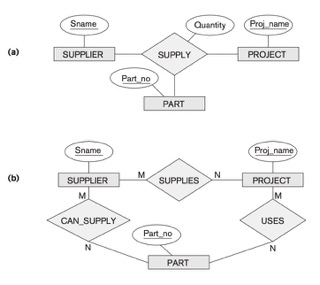
\includegraphics[scale=0.7]{relazlivalt.jpeg}
\caption{Relazione di livello alto} 
\label{relazlivalt}
\end{figure}
